\documentclass[a4paper,10pt,oneside,final,titlepage,onecolumn]{article}

\usepackage{ucs}
\usepackage[portuguese]{babel}
\usepackage[utf8x]{inputenc}
\usepackage[T1]{fontenc}
\usepackage{textcomp}
\usepackage{graphicx}
\usepackage{placeins}

\usepackage{listings}
\usepackage{color}

\definecolor{dkgreen}{rgb}{0,0.6,0}
\definecolor{gray}{rgb}{0.5,0.5,0.5}
\definecolor{mauve}{rgb}{0.58,0,0.82}

\lstset{frame=tb,
  language=bash,
  aboveskip=3mm,
  belowskip=3mm,
  showstringspaces=false,
  columns=flexible,
  basicstyle={\scriptsize\ttfamily},
  numbers=none,  
  breaklines=true,
  breakatwhitespace=true
  tabsize=3
}



\title{Exercício 4 de MC833 --- Programação em Redes de Computadores}
\author{Raul Rabelo Carvalho, 105607, turma A}



\begin{document}



\maketitle



\section{}
\paragraph{}A figura \ref{print-ipport-client} mostra o cliente imprimindo na saída padrão o endereço IP e a porta associados à conexão pelo sistema operacional. O servidor está sendo executado no \emph{host} \verb|guns.lab.ic.unicamp.br:10101| (\verb|143.106.16.5:10101)| e o cliente, no \emph{host} em \verb|143.106.16.163|. O endereço IP e a porta impressas pelo cliente são confirmadas pela linha destacada na saída do comando \verb|netstat -tun|.
\begin{figure}[!ht]
  \caption{Cliente imprimindo o endereço IP e a porta.}
  \centering
  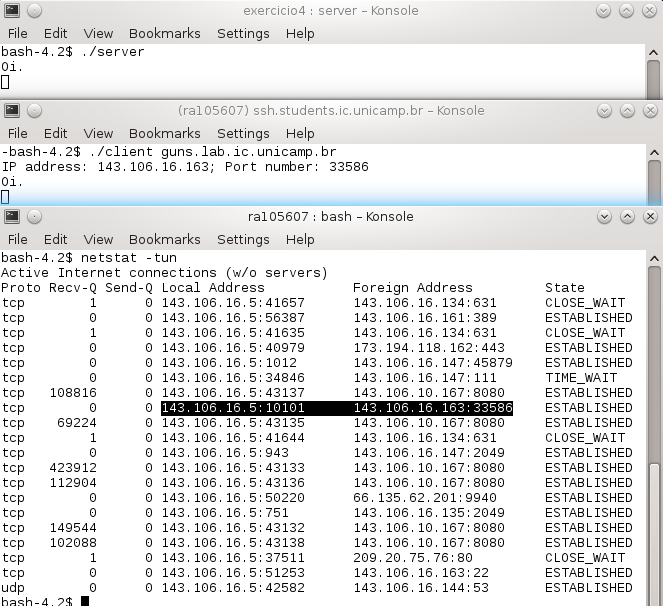
\includegraphics[width=117mm]{images/print-ipport-client.png}
  \label{print-ipport-client}
\end{figure}



\FloatBarrier
\section{}
\paragraph{}A figura \ref{print-ipport-server} mostra tanto o cliente como o servidor imprimindo na saída padrão o endereço IP e a porta associados ao cliente pelo sistema operacional local. O servidor está sendo executado no \emph{host} \verb|guns.lab.ic.unicamp.br| (no endereço IP \verb|143.106.16.5)|, mas agora na porta 10102, e o cliente, no \emph{host} em \verb|143.106.16.163|. O endereço IP e a porta impressas por ambos programas são confirmadas pela linha destacada na saída do comando \verb|netstat -tun|.
\begin{figure}[!ht]
  \caption{Servidor imprimindo o endereço IP e a porta.}
  \centering
  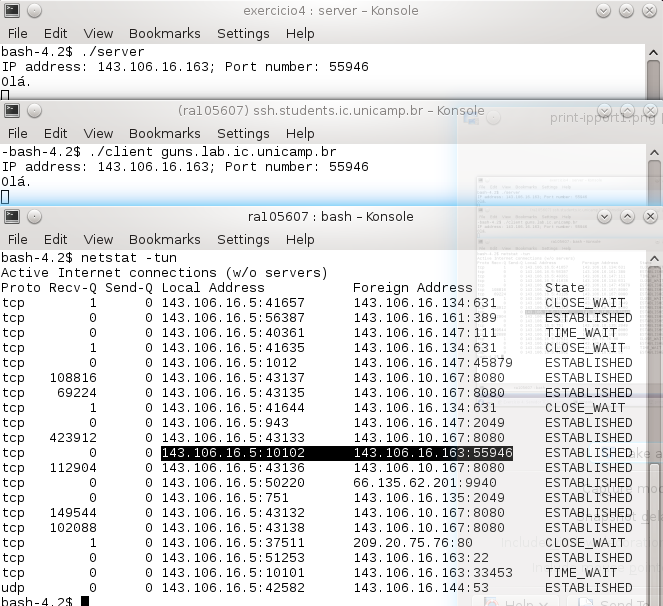
\includegraphics[width=117mm]{images/print-ipport-server.png}
  \label{print-ipport-server}
\end{figure}



\FloatBarrier
\section{}
\paragraph{}O código pertinente ao servidor de múltiplas conexões segue abaixo, comentado.
\begin{lstlisting}
	while(1) {
		/* aceita a conexao de um cliente por um socket novo new_s */
		if ((new_s = accept(s, (struct sockaddr *)&sin, &len)) < 0) {
			perror("simplex-talk: accept");
			exit(EXIT_FAILURE);
		}
		/* faz o fork do processo */
		child_pid = fork();
		if (child_pid < 0) {
			perror("simplex-talk: fork");
			exit(EXIT_FAILURE);
		}
		/* caso o processo seja o filho */
		if (child_pid == 0) {
			/* fecha o socket que esta' esperando por novos clientes */
			close(s);
			/* coleta as informacoes do socket e imprime na stdout */
			so_len = sizeof(so);
			if (getpeername(new_s, (struct sockaddr *)&so, &so_len) < 0) {
				perror("simplex-talk: getpeername");
				close(s);
				exit(EXIT_FAILURE);
			}
			inet_ntop(AF_INET, &(so.sin_addr), so_addr, INET_ADDRSTRLEN);
			printf("IP address: %s; Port number: %d\n", so_addr, ntohs(so.sin_port));
			/* entra em loop imprimindo as mensagens do cliente */
			while (len = recv(new_s, buf, sizeof(buf), 0)) {
				fputs(buf, stdout);
			}	
		}
		/* caso o processo seja o pai, fecha o novo socket */
		close(new_s);	
	}
\end{lstlisting}



\FloatBarrier
\section{}
\paragraph{}Segue abaixo o trecho de código a ser explicado.
\begin{lstlisting}
for (;;) {
   connfd = Accept (listenfd,...);

   if ( (pid=Fork()) == 0) {
      Close(listenfd);
      doit(connfd); // Faz alguma operacao no socket
      Close(connfd);
      exit(0);
   }
   Close(connfd);
}
\end{lstlisting}
\paragraph{}Após a execução do \verb|fork|, existem dois processos diferentes com \verb|pid|s diferentes. O processo-pai tem esta variável definida com o número do processo-filho, portanto, ele não executa o bloco do \verb|if|, vindo somente a fechar o \emph{socket} \verb|connfd| enquanto continua a aguardar novas conexões no \emph{socket} \verb|listenfd|. Já no caso do processo-filho, sua variável \verb|pid| é zero, então, o bloco do \verb|if| é executado. Dentro do bloco, o \emph{socket} \verb|listenfd| é fechado imediatamente, mas isso não afeta o funcionamento geral do sistema, já que o processo-pai continua a escutar neste \emph{socket}. O processo-filho, deste modo, ficou encarregado da conexão com o cliente pelo \emph{socket} \verb|connfd|, o qual só é encerrado depois de executar as operações desejadas pelo cliente.



\FloatBarrier
\section{}
\paragraph{}Podemos comprovar que os processos extras que o servidor cria são seus filhos usando a \emph{tree view} do programa \verb|htop|, o que é uma versão com mais recursos da ferramenta \verb|top|. Na figura \ref{htop}, vê-se que existem dois processos-filhos de um processo \verb|server| sendo executando no \emph{shell} \verb|bash| em um \verb|konsole| (terminal virtual do KDE).
\begin{figure}[!ht]
  \caption{htop mostrando os processos do servidor.}
  \centering
  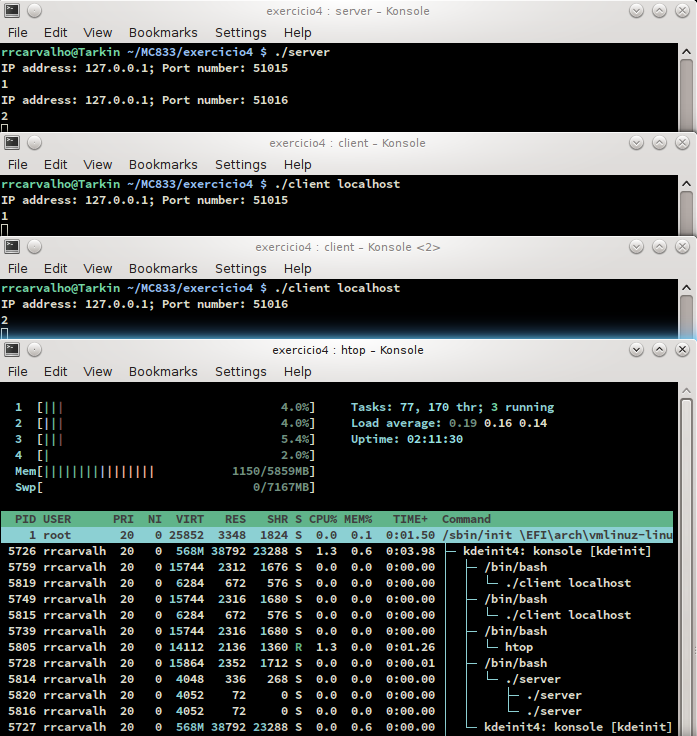
\includegraphics[width=117mm]{images/htop.png}
  \label{htop}
\end{figure}



\FloatBarrier
\section{}
\paragraph{}Para verificar quais dos lados da conexão entra no estado \verb|TIME_WAIT|, foi feita uma modificação no cliente para ele este encerre a conexão após a entrada da palavra \verb|exit|. Assim, o cliente será o lado que iniciará o encerramento da conexão. O comando para verificação foi \verb|netstat -tun|.
\begin{figure}[!ht]
  \caption{Saída do netstat.}
  \centering
  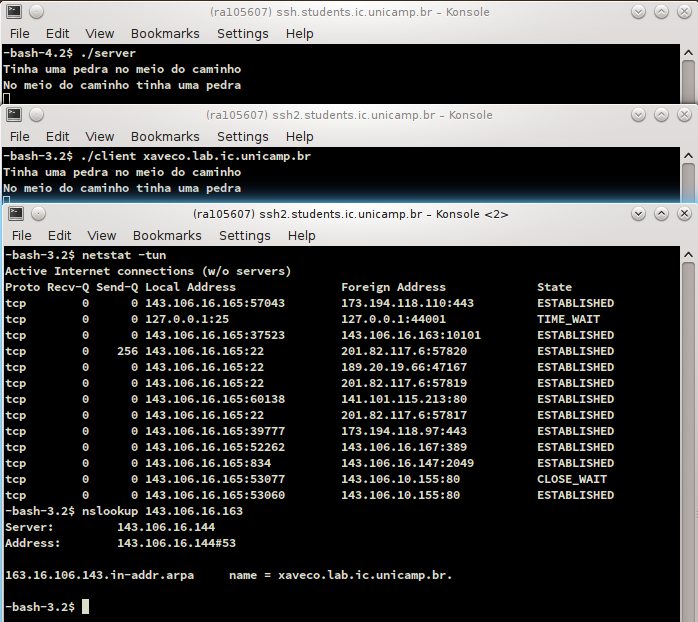
\includegraphics[width=117mm]{images/netstat.png}
  \label{netstat}
\end{figure}
\paragraph{}Como visto na figura \ref{netstat}, o lado que inicia o encerramento da conexão que entra em \verb|TIME_WAIT|. Isso é condizente com a máquina de estados do protocolo TCP\footnote{Stevens, W. Richard. UNIX Network Programming. 2nd Edition, pp. 40-41}. O estado \verb|TIME_WAIT| existe garantir o encerramento adequado da conexão TCP. O cliente fica neste estado por duas vezes o MSL (\emph{maximum segment lifetime}), caso o ACK que ele enviou em resposta ao FIN do servidor (note que o cliente inciou o encerramento enviando um FIN ao servidor que foi por este respondido com um ACK seguido de un FIN) não seja entregue a este. O cliente precisa manter o estado da conexão para caso o servidor re-envie seu FIN.



\end{document}
